\documentclass[onecolumn,draftclsnofoot, 10pt, compsoc]{IEEEtran}

\usepackage{graphicx}
\usepackage[section]{placeins}
\usepackage{caption}

\usepackage{amssymb}                                         
\usepackage{amsmath}                                         
\usepackage{amsthm}                                

\usepackage{alltt}                                           
\usepackage{float}
\usepackage{color}
\usepackage{url}

\usepackage{balance}
\usepackage[TABBOTCAP, tight]{subfigure}
\usepackage{enumitem}
\usepackage{pstricks, pst-node}
\usepackage{url}
\usepackage{setspace}

\usepackage{etoolbox}
\AtBeginEnvironment{quote}{\singlespacing\vspace{-\topsep}\small}

%\input{pygments.tex}

\usepackage{geometry}
\geometry{left=0.75in,right=0.75in,top=0.75in,bottom=0.75in}
\parindent = 0.0 in
\parskip = 0.1 in


\def \ParSpace{\vspace{.75em}}
\def \GroupNumber{		17}
\def \Jeremy{			Jeremy Fischer}
\def \Class{		Parallel Programming}
\def \Assn{		Project 3: False Sharing}
\def \School{	Oregon State University}
\def \Professor{		Matthew Meyn}

\newcommand{\cred}[1]{{\color{red}#1}}
\newcommand{\cblue}[1]{{\color{blue}#1}}

\newcommand{\NameSigPair}[1]{
		\par
		\makebox[2.75in][r]{#1} \hfil 	\makebox[3.25in]{\makebox[2.25in]{\hrulefill} \hfill			
		\makebox[.75in]{\hrulefill}}
		\par\vspace{-12pt} \textit{
			\tiny\noindent
			\makebox[2.75in]{} \hfil		
			\makebox[3.25in]{
				\makebox[2.25in][r]{Signature} \hfill	\makebox[.75in][r]{Date}
			}
		}
}










%%%%%%%%%%%%%%%%%%%%%%%%%%%%%%%%%%%%%%%
\begin{document}
\begin{titlepage}
    \pagenumbering{gobble}
    \begin{singlespace}
    	
\includegraphics[height=4cm]{coe.eps}
        \hfill  
        \par\vspace{.2in}
        \centering
        \scshape{
            \vspace{.5in}
            \textbf{\Large\Assn}\par
            \textbf{\large\Class}\par
            \large{
            	\today \\Spring Term
        	}
            \vfill
            {\large Prepared for}\par
            \huge \School\par
            \vspace{5pt}
            {\Large{\Professor}\par}
            {\large Prepared by }\par
           % Group\GroupNumber\par
            \vspace{5pt}
            {\Large
                {\Jeremy}\par
            }
            \vspace{20pt}
        }

    \end{singlespace}
\end{titlepage}
\newpage
\pagenumbering{arabic}

% 7. uncomment this (if applicable). Consider adding a page break.
%\listoffigures
%\listoftables
\clearpage







	\section{Tell what machine you ran this on}	
	I ran this test on a 2015 Macbook Pro, 2.2 GHz Intel Core i7, 16 GB 1600 MHz DDR3.
	
	
	\section{Results}
	The below table represents Fix \#1. The bold numbers in the first row are the number of padding fields, the bold numbers in the first column are the number of threads, and the values in the middle are the speedups.
	
	\begin{figure}[H]
		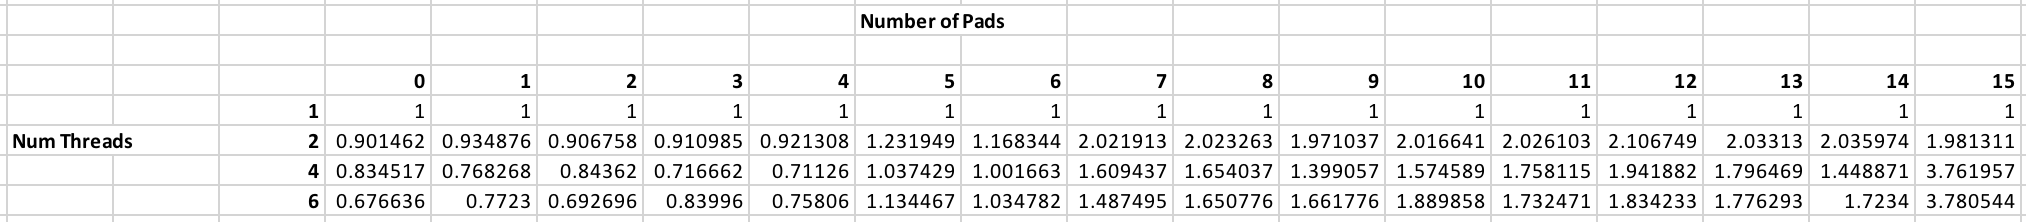
\includegraphics[width=18cm, height=2cm]{paddingTable}
		\centering
		\caption{Fix \#1}
	\end{figure}

	\begin{figure}[H]
		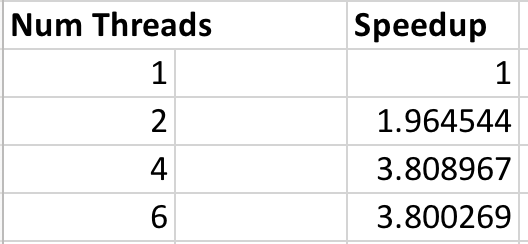
\includegraphics[width=6cm]{fix2}
		\centering
		\caption{Fix \#2}
	\end{figure}

	\begin{figure}[H]
		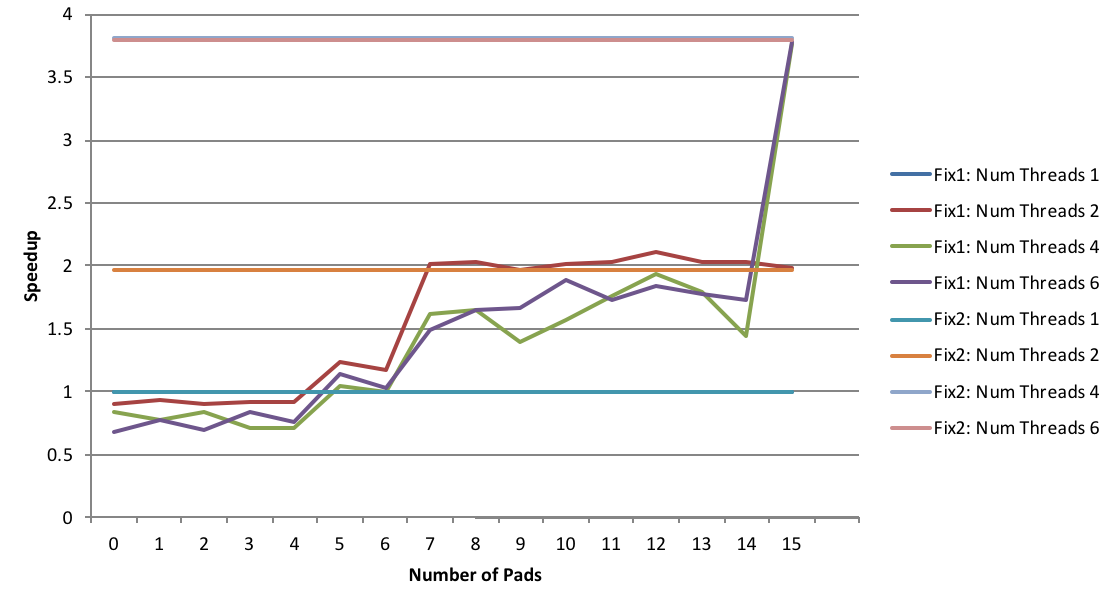
\includegraphics[width=18cm]{Graph}
		\centering
		\caption{Fix \#1 and Fix \#2 speedups per number of threads}
	\end{figure}


\clearpage

\section{What patterns are you seeing in the speeds?}
	Fix \#1 is very interesting. The speedup with one thread is, or course, one. But, when the number of threads is greater than one, the speedups dip below one from 0 - 5 pads, as in, there is a decrease in speed. When there are two threads the speedup flattens out after seven pads, and when there are four and six threads, the speedup doesn't settle down until there is a padding of 15. 
	
	When Fix \#2 is used, the speedup for all numbers of threads is static at about the same amount as its counterpart's peak in Fix \#1.
	
\section{Why do you think it is behaving this way?}
	For the Fix \#1 curves, when the number of threads is greater than one with the number of pads between 0 and 4, the speedup is less than one. This is due to the false sharing that is taking place. All of the threads are sharing the same cache line, and thus a bad performance is occurring due to the repetitive false sharing. The little hop ups in speedup is due to a value in the array moving down to a new cache line due to the number of pads pushing it off the current line. Finally, with the number of pads equal to 15, the performance is up where it should be because all four array slots are on their own cache line, thus reducing the false sharing.
	
	For the Fix \#2 curves, they are static at about the same amount as their counterpart's peak in Fix \#1 due to the use of a private variable taking on the Arr[\textit{idx}].value. That private value lives in the individual thread's stack frame, so there is no repeated false sharing because the private variable only writes back to the array that is shared by all threads after the thread is done computing what it needs to compute. As you can see by the graph, this greatly improves the performance by tremendously reducing the amount of false sharing.



\end{document}